\subsubsection{Purpose}
After 5 minutes from the end of the ride, that is the time the system gives to the user to plug the car to the grid, the systems computes the charge that has to be applied to the driver. The system takes into accounts discounts and additional charges as well as regular charges for the car utilization. After that, the system can manage the payment by sending a request to the payment handler (see section \ref{man_pay} for further details). If no errors occur, the system updates the rides history of the user.

\subsubsection{Scenario 1}
Rick has just safely parked his car into the boundaries of the Safe Area. He exits the car and end his ride. After 5 minutes, since during the ride no discounts/additional charges situations have been detected, the system charges him the only car utilization fare.

\subsubsection{Scenario 2}
During the ride performed by Carl, the systems has detected some additional charges situations. As soon as he parks and locks the car and 5 minutes pass, the system charges Carl not only the simple utilization fare, but takes also into account the additional charges.

\subsubsection{Use-case}
The apply charges use-case is shown in Table \ref{apply_charges_uc}. \\
The activity diagram showing the event flow is shown in figure \ref{app_charges_act}

\subsubsection{Functional requirements}
\begin{enumerate}
\item The system must take into account discounts and additional charges when the final charge is calculated;
\item The system shall apply charges to the user within 5 minutes from the end of the ride.
\end{enumerate}

\begin{table}[H]
\begin{center}
\begin{tabular}{p{0.3\textwidth} | p{0.7\textwidth}}
\hline
Actor & Logged user\\
\hline
Goal & Goal 6\\
\hline
Input Condition & The user's ride comes to an end and 5 minutes pass.\\
\hline
Event Flow & 
\begin{enumerate}
\item The system calculate the amount of money the driver has to pay taking into account discounts and additional charges;
\item The system manages the payment.
\end{enumerate} \\
\hline
Output Condition & The system updates rides history of the user.\\
\hline
Exception & If an error occurs at point 2 of the Event Flow, the system does not update the rides history and waits for the user's payment.\\
\hline
\end{tabular}
\end{center}
\caption{Apply charges use-case}
\label{apply_charges_uc}
\end{table}

\begin{figure}[H]
\begin{center}
		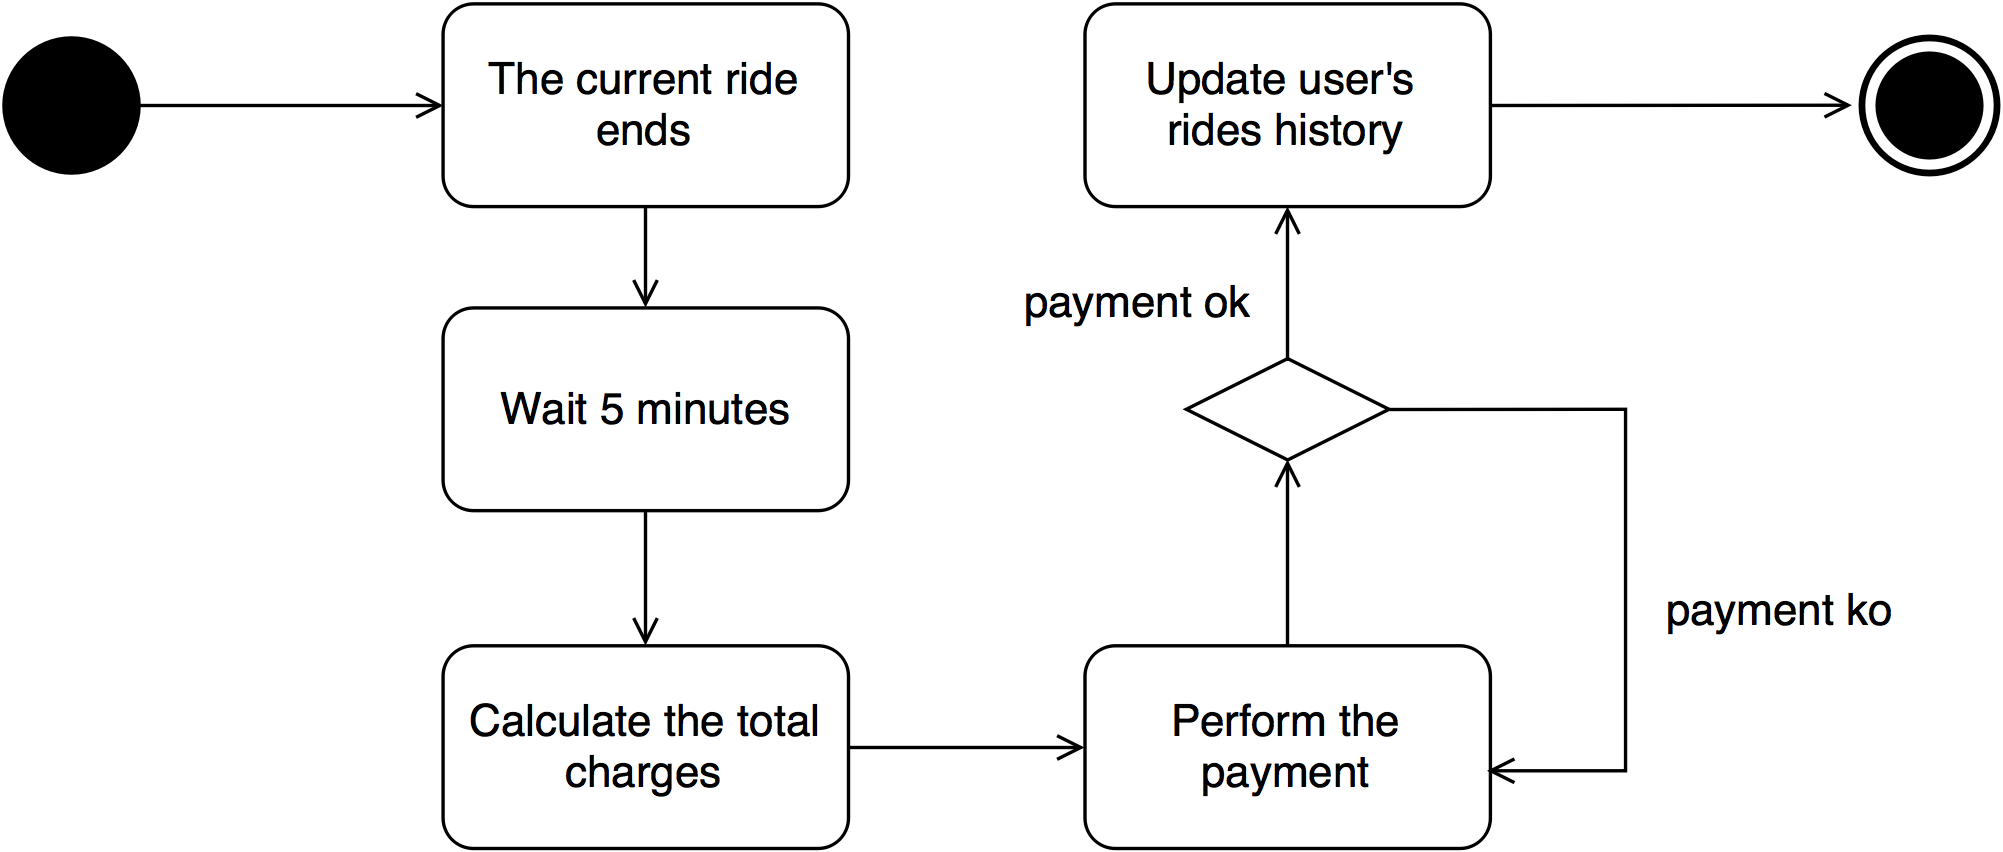
\includegraphics[width=\textwidth]{./specific_requirements/features/diagrams/apply_charges_activity.png}
		\caption{Activity diagram of the apply charges use-case from the system point of view.}
		\label{app_charges_act}
\end{center}
\end{figure}